\subsection{Image-to-Image Schrödinger Bridge}
\label{sec:i2sb}
Image inpainting is the process of restoring or completing portions of an image, the second phase in our watermark removal pipeline. After identifying the specific watermark location, image inpainting techniques can also be used to remove the visible watermarks \cite{huang2004attacking}. Thus, attention-guided inpainting methods, such as Partial Convolution \cite{liu2018image}, Contextual Attention \cite{yu2018generative} and Gated Convolution \cite{Yu:2018uw} are applicable to this task. Recently, Generative Adversarial Networks (GAN) \cite{goodfellow2014generative} and Image-to-Image Schrödinger Bridge (I$^2$SB) \cite{liu2023i2sb} are developed as state-of-the-art works. GAN trains two adversarial networks. A generator $G$ generates a sample $X$ as close to the dataset as possible and a discriminator $D$ labels the probability that $X$ is generated by $G$, not from the real dataset. Through adversarial training, $G$ and $D$ converge to the Nash equilibrium. On the other hand, I$^2$SB is developed recently from conditional diffusion models, using a tractable class of Schrödinger Bridge. As diffusion models are shown to beat GAN on image generation tasks \cite{dhariwal2021diffusion}, we present I$^2$SB as the main approach to our image inpainting task.

\begin{figure}[t]
  \begin{center}
    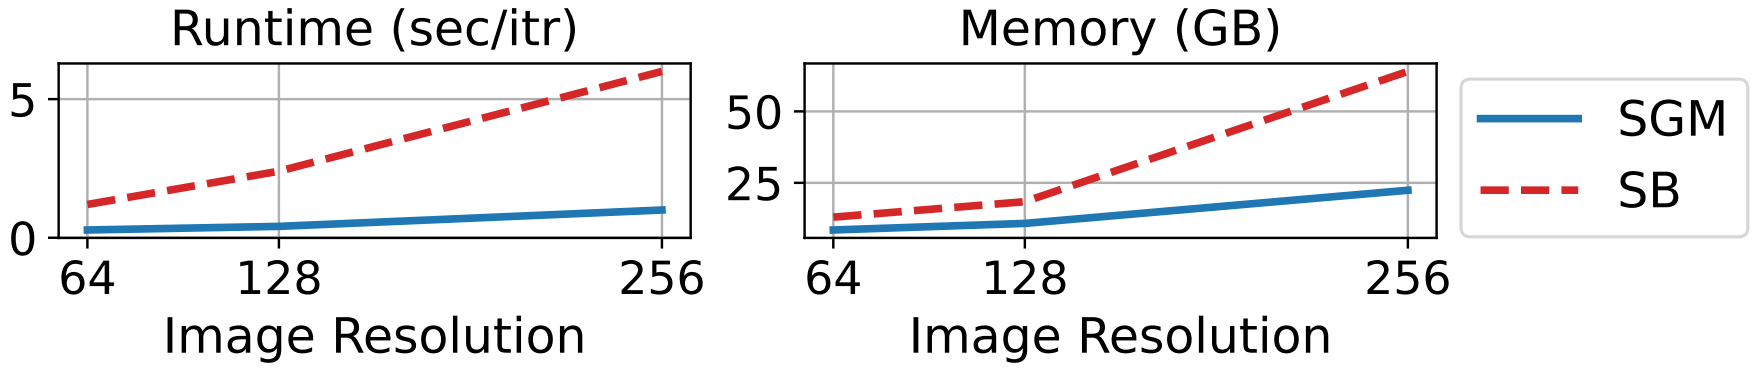
\includegraphics[width=0.85\columnwidth]{img/complexity.png}
    \caption[Complexity of SGM and SB]{
      Complexity of SGM and SB \cite{chen2021likelihood} On 256$\times$256 resolution, SB is 6$\times$ slower and consumes 3$\times$ memory.
    }
    \label{figure:complexity}
  \end{center}
\end{figure}

\begin{figure}[t]
    \centering
    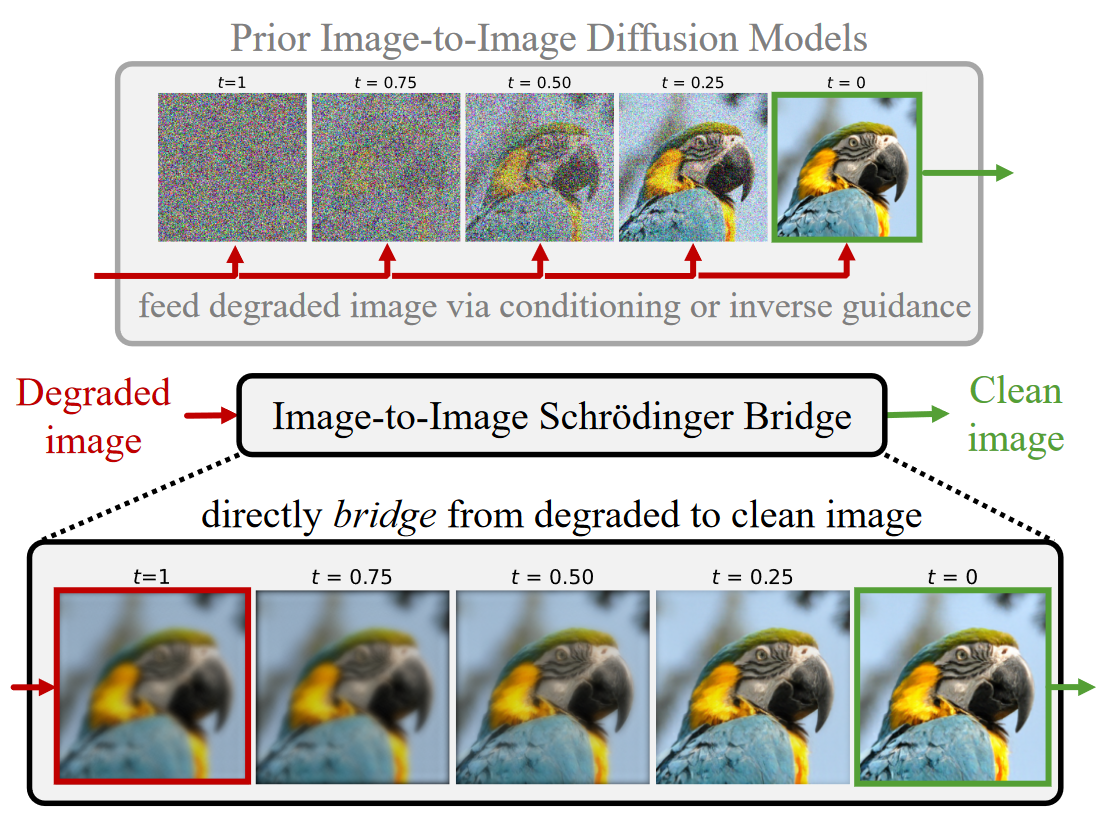
\includegraphics[width=0.6\linewidth]{diffusion-vs-sb.png}
    \caption{Difference between predominant non-conditional diffusion models and I$^2$SB}
    \label{figure:diffusion-vs-sb}
\end{figure}

Figure \ref{figure:complexity} illustrates the complexity of Likelihood Training of Schrödinger Bridge \cite{chen2021likelihood}, a previous SB approach (see Section \ref{section:diffusion-models}) for image generation. I$^2$SB employs a tractable class of SB for better training efficiency, cognizing that the train dataset is Dirac Delta distributed. The difference between non-conditional diffusion models and I$^2$SB can be seen in Figure \ref{figure:diffusion-vs-sb}. Non-conditional models generates a new sample in the image dataset distribution from the Gaussian noise, while I$^2$SB convert an image in the degraded distribution to an image in the clear distribution. 

\begin{sbtheorem}[Tractable SB with the Dirac Delta Boundary]
  \label{theo-dirac}
  Let $p(\cdot,0) := \delta_a(\cdot)$ be the Dirac delta distribution centered at $a\in\RR^d$. Then, the initial distributions in (\ref{equation:sde-psihat}) and (\ref{equation:sde-psi}) are given by
  \begin{equation}
    \label{equation:sb-dirac}
    \hat{\Psi}(\cdot,0)= \delta_A(\cdot), \Psi(\cdot,1)=\dfrac{p(\cdot, 1)}{\hat{\Psi}(\cdot,1)}.
  \end{equation}
\end{sbtheorem}

The Dirac delta assumption also implicitly appears in the denoising objective, which first computes the target $\nabla\log p(\xbf_t,t|\xbf_0=a)$ for each data point $a$, as the score between $\delta_{a}(\cdot)$ and Gaussian, then averages over $\xbf_0 {\sim} p_\A$. In this vein, Theorem \ref{theo-dirac} adopts the same boundary $\delta_{a}(\cdot)$ on one side and generalizes the other side from Gaussian to arbitrary $p_\B$. Based on the details provided in Table \ref{table:comp_diff}, it becomes evident that employing Theorem \ref{theo-dirac} enables us to transform the Schrödinger Bridge (SB) model, which is challenging to handle at $\nabla\log\hat{\psi}$ and demands substantial time and resources for training. With our model I$^2$SB, utilizing the degraded dataset allows us to generate a pair of information from the clean image. Consequently, the term $\nabla\log\hat{\psi}$ becomes manageable, enabling us to calculate the score with reduced resource requirements.


\begin{table}[H]
  \caption[Comparison of different diffusion models in boundary distributions and tractability]{
    Comparison of different diffusion models in boundary distributions and tractability of forward and backward drifts. Note that I$^2$SB requires paired information compared to standard SB}
  \label{table:comp_diff}
  \label{table:comp}
  \vskip 0.05in
  \begin{center}
    \begin{small}
      \begin{tabular}{rclcc}
        \toprule
        \textbf{Model} & \textbf{$\mathbf{p(\xbf_0)}$} & \textbf{$\mathbf{p(\xbf_1)}$} & \textbf{$\mathbf{\gradlog \Psi}$} & \textbf{$\mathbf{\gradlog \Psihat}$} \\ [0.5ex]
        \midrule
        (C)SGM
                       & $p_\A$                        & $\N(0,I)$                     & 0                                 & tractable                            \\[0.5ex]
        \textbf{I$^2$SB}
                       & $p_\A$                        & $p_\B(\cdot|\xbf_0)$          & intractable                       & tractable                            \\[0.5ex]
        SB
                       & $p_\A$                        & $p_\B(\cdot)$                 & intractable                       & intractable                          \\
        \bottomrule
      \end{tabular}
    \end{small}
  \end{center}
  \vskip -0.15in
\end{table}

